\section{Estimación de Pose 3D}

En la sección \ref{sec:taxonomy}, previamente mencionamos que la estimación de pose puede hacerse
en dos etapas. La primer etapa encargada de predecir las poses en 2 dimensiones y la segunda en
realizar la predicción a 3 dimensiones a partir de los resultados de la etapa anterior. Este esquema
de predicción y entrenamiento fue uno de los primeros propuestos por J. Martinez
\cite{DBLP:journals/corr/MartinezHRL17}. La tarea de estimación de pose 2D está relativamente madura
con resultados bastante precisos, así que suena prudente aprovechar estos modelos ya existentes para
resolver un primera parte del problema. Así, Martinez entrena un nuevo modelo que utiliza esta
información para generar la poses en un dimensión más alta, dejando los problemas como lidiar con las
escenas de fondo, iluminación, color y texturas de las ropas, color de piel o diversas imperfecciones
de las imágenes, en la primer etapa.

\begin{figure}[!ht]
    \centering
    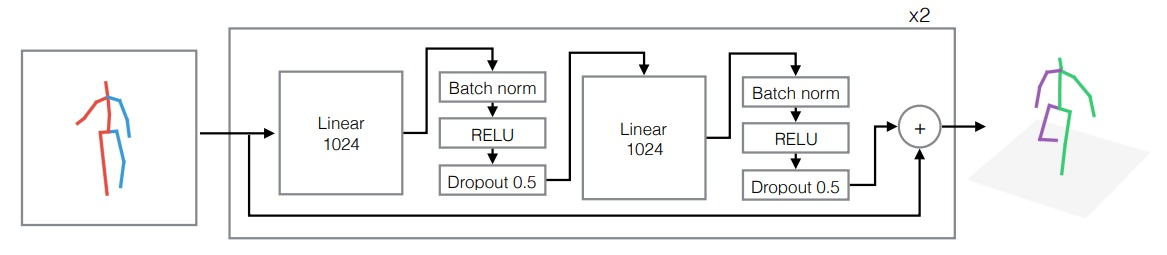
\includegraphics[width=.9\textwidth]{Chapters/3. Trans-HPE/img/martinez_model.jpeg}
    \caption[2D a 3D model]{Modelo usado por J. Martinez \cite{DBLP:journals/corr/MartinezHRL17}
    basado en una simple red neuronal multicapa usando batch normalization, dropout, Rectified
    Linear Units y residual connections.}
\label{fig:model_martinez}
\end{figure}

En la figura \ref{fig:model_martinez} se muestra el modelo usado por J. Martinez. Los datos de entrada
son las posiciones de las articulaciones del cuerpo humano, estos son incrementados de dimensión a
1024 usando la primer capa lineal, posteriormente pasa a un proceso de normalización por lotes
y son activados con una función \textit{RELU} con dropout de 50 por ciento. La salida de este modelo
es proyectada para tener una dimensión de $3n$ con $n$ como el número de articulaciones, representando
puntos en un espacio de 3 dimensiones.

Por otra parte,
Leer y explicar lo que hace martinez
y lo que hace el otro tipejo

- Dos proyectos
- el de gonzales
- el otro que jaló mejor

- Proyecto del tipo que usa transformers

Proyecto enfocado solo en Estimación de pose 2D HPE y 3D HPE considerando un solo objetivo SPPE

Para el primer caso solo martinez solo se enfoca en el segundo stage de la estimación de pose
no se usa un modelo end-to-end sino que aprovecha los modelos ya creados para estimación de pose
en 2d y

\section{Arquitecturas de Estimación 2D y 3D}

Explicar las arquitecturas usadadas
- la de martinez
- La del transformer
- La que funciona

\section{Modificación a transformers - Usando cabezas de Atención flexibles}

\section{Evaluación y comparativas}
